\begin{appendices}
\chapter{Detailed Description of the 20Newsgroups-End2End architecture}
\begin{tabularx}{\textwidth}[!h]{X X X}
	% \caption{MNIST-Lenet-FCN}
	\multicolumn{3}{X}{\textbf{Newsgroup-End2End}}\\
	\\
	\hline
	\endhead
	\textbf{Sequential Layer Defaults} & \textbf{Embedding} & input dimension = 61188\\
	& & input length = 200\\
	& & output dimension = 300\\
	& \textbf{1D Convolution} & filters = 3\\
	& \textbf{1D Average Pooling} &\\
	& \textbf{Dropout} & rate = 0.5\\
	& \textbf{1D Global Average Pooling} &\\
	%\noalign{\hrule height 2pt}
	\hline
	\textbf{Input} & output dimension & [61188|200]\\
	[8pt]
	\textbf{Sequential A1} & input from & Input\\
	& \textbf{1D Convolution} & kernel size = 1\\
	& \textbf{1D Average Pooling} & pool size = 2\\
	& output dimension & 3\\
	[8pt]
	\textbf{Sequential A2} & input from & Input\\
	& \textbf{1D Convolution} & kernel size = 4\\
	& \textbf{1D Average Pooling} & pool size = 2\\
	& output dimension & 3\\
	[8pt]
	\textbf{Sequential A3} & input from & Input\\
	& \textbf{1D Convolution} & kernel size = 7\\
	& \textbf{1D Average Pooling} & pool size = 2\\
	& output dimension & 3\\
	[8pt]
	\textbf{Sequential A4} & input from & Input\\
	& \textbf{1D Convolution} & kernel size = 10\\
	& \textbf{1D Average Pooling} & pool size = 2\\
	& output dimension & 3\\
	[8pt]
	\textbf{Sequential A5} & input from & Input\\
	& \textbf{1D Convolution} & kernel size = 13\\
	& \textbf{1D Average Pooling} & pool size = 2\\
	& output dimension & 3\\
	[8pt]
	\textbf{Sequential A6} & input from & Input\\
	& \textbf{1D Convolution} & kernel size = 16\\
	& \textbf{1D Average Pooling} & pool size = 2\\
	& output dimension & 3\\
	[8pt]
	\textbf{Sequential A7} & input from & Input\\
	& \textbf{1D Convolution} & kernel size = 19\\
	& \textbf{1D Average Pooling} & pool size = 2\\
	& output dimension & 3\\
	[8pt]
	\textbf{Sequential A8} & input from & Input\\
	& \textbf{1D Convolution} & kernel size = 22\\
	& \textbf{1D Average Pooling} & pool size = 2\\
	& output dimension & 3\\
	[8pt]
	\textbf{Sequential B1} & input from & Input\\
	& \textbf{1D Convolution} & kernel size = 1\\
	& \textbf{1D Average Pooling} & pool size = 7\\
	& output dimension & 3\\
	[8pt]
	\textbf{Sequential B2} & input from & Input\\
	& \textbf{1D Convolution} & kernel size = 4\\
	& \textbf{1D Average Pooling} & pool size = 7\\
	& output dimension & 3\\
	[8pt]
	\textbf{Sequential B3} & input from & Input\\
	& \textbf{1D Convolution} & kernel size = 7\\
	& \textbf{1D Average Pooling} & pool size = 7\\
	& output dimension & 3\\
	[8pt]
	\textbf{Sequential B4} & input from & Input\\
	& \textbf{1D Convolution} & kernel size = 10\\
	& \textbf{1D Average Pooling} & pool size = 7\\
	& output dimension & 3\\
	[8pt]
	\textbf{Sequential B5} & input from & Input\\
	& \textbf{1D Convolution} & kernel size = 13\\
	& \textbf{1D Average Pooling} & pool size = 7\\
	& output dimension & 3\\
	[8pt]
	\textbf{Sequential B6} & input from & Input\\
	& \textbf{1D Convolution} & kernel size = 16\\
	& \textbf{1D Average Pooling} & pool size = 7\\
	& output dimension & 3\\
	[8pt]
	\textbf{Sequential B7} & input from & Input\\
	& \textbf{1D Convolution} & kernel size = 19\\
	& \textbf{1D Average Pooling} & pool size = 7\\
	& output dimension & 3\\
	[8pt]
	\textbf{Sequential B8} & input from & Input\\
	& \textbf{1D Convolution} & kernel size = 22\\
	& \textbf{1D Average Pooling} & pool size = 7\\
	& output dimension & 3\\
	[8pt]
	\textbf{Concatenate} & input from & Sequential A1\\
	& & Sequential A2\\
	& & Sequential A3\\
	& & Sequential A4\\
	& & Sequential A5\\
	& & Sequential A6\\
	& & Sequential A7\\
	& & Sequential A8\\
	& & Sequential B1\\
	& & Sequential B2\\
	& & Sequential B3\\
	& & Sequential B4\\
	& & Sequential B5\\
	& & Sequential B6\\
	& & Sequential B7\\
	& & Sequential B8\\
	& output dimension & 48\\
	[8pt]
	\textbf{Dropout} & input from & Concatenate\\
	& rate & 0.5\\
	[8pt]
	\textbf{Dense} & input from & Dropout\\
	& output dimension & 20\\
	& activation & softmax\\
	\hline
	%\noalign{\hrule height 2pt}
\end{tabularx}


%\chapter{A history of neural networks}
%\begin{itemize}
%	\item 1. wave: ~ 1955-1970
%	\item 2. wave: ~ 1985-2000 \(?\)
%	\item 3. wave: ~ ??? 
%\end{itemize}
%\begin{figure}
%	\centering
%	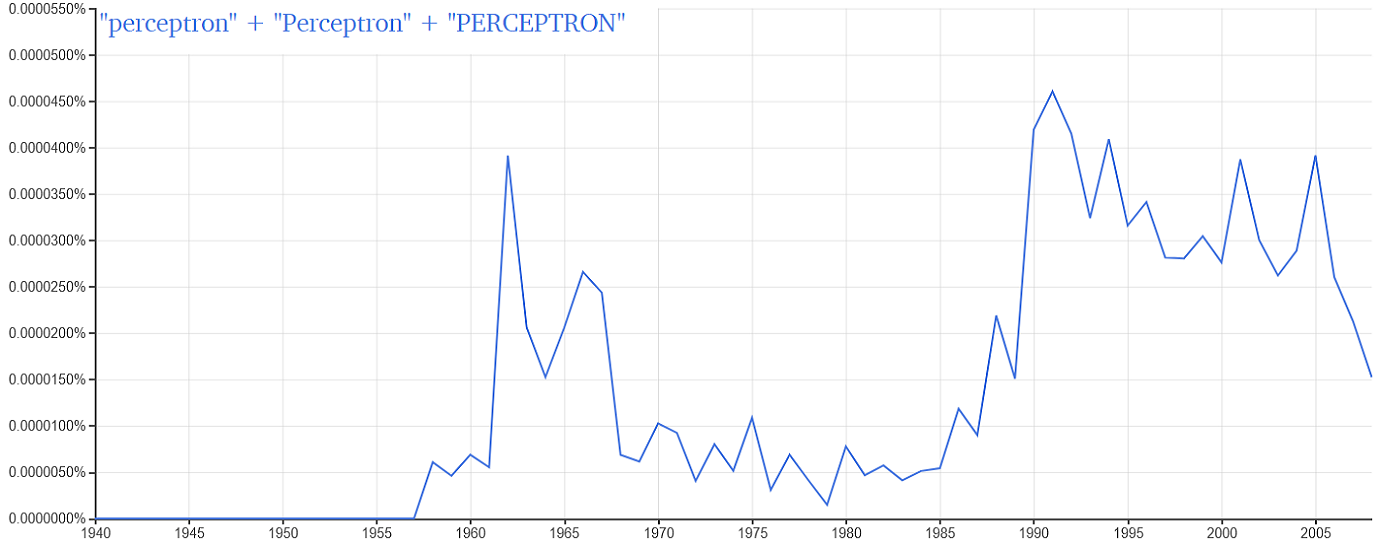
\includegraphics[height=150px]{gfx/NGrams_Perceptron.png}
%	\caption{Relative amount of occurences of the word "Perceptron" in published books between 1940 and 2009}
%\end{figure}
%\begin{figure}
%	\centering
%	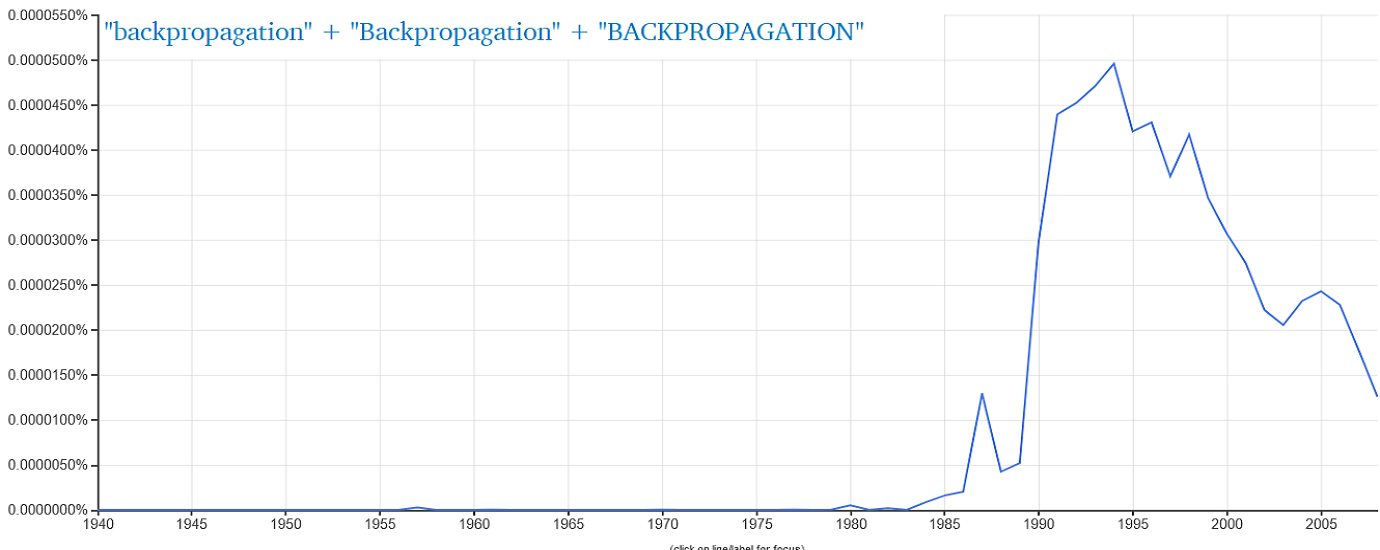
\includegraphics[height=150px]{gfx/NGrams_Backpropagation.png}
%	\caption{Relative amount of occurences of the word "Backpropagation" in published books between 1940 and 2009}
%	\label{fig:NGBackprop}
%\end{figure}

\end{appendices}